\section*{Chapitre \ref{chap:simple}}
\addcontentsline{toc}{section}{Chapitre \protect\ref{chap:simple}}

\begin{solution}{2.1}
    \begin{enumerate}
    \item Voir la figure \ref{fig:simple:base}. Remarquer que l'on
      peut, dans la fonction \texttt{plot}, utiliser une formule pour
      exprimer la relation entre les variables.
      \begin{figure}
        \centering
\begin{knitrout}
\definecolor{shadecolor}{rgb}{0.969, 0.969, 0.969}\color{fgcolor}\begin{kframe}
\begin{alltt}
\hlstd{x}\hlkwb{<-}\hlkwd{c}\hlstd{(}\hlnum{65}\hlstd{,} \hlnum{43}\hlstd{,} \hlnum{44}\hlstd{,} \hlnum{59}\hlstd{,} \hlnum{60}\hlstd{,} \hlnum{50}\hlstd{,} \hlnum{52}\hlstd{,} \hlnum{38}\hlstd{,} \hlnum{42}\hlstd{,} \hlnum{40}\hlstd{)}
\hlstd{y}\hlkwb{<-}\hlkwd{c}\hlstd{(}\hlnum{12}\hlstd{,} \hlnum{32}\hlstd{,} \hlnum{36}\hlstd{,} \hlnum{18}\hlstd{,} \hlnum{17}\hlstd{,} \hlnum{20}\hlstd{,} \hlnum{21}\hlstd{,} \hlnum{40}\hlstd{,} \hlnum{30}\hlstd{,} \hlnum{24}\hlstd{)}
\hlkwd{plot}\hlstd{(y} \hlopt{~} \hlstd{x,} \hlkwc{pch} \hlstd{=} \hlnum{16}\hlstd{)}
\end{alltt}
\end{kframe}
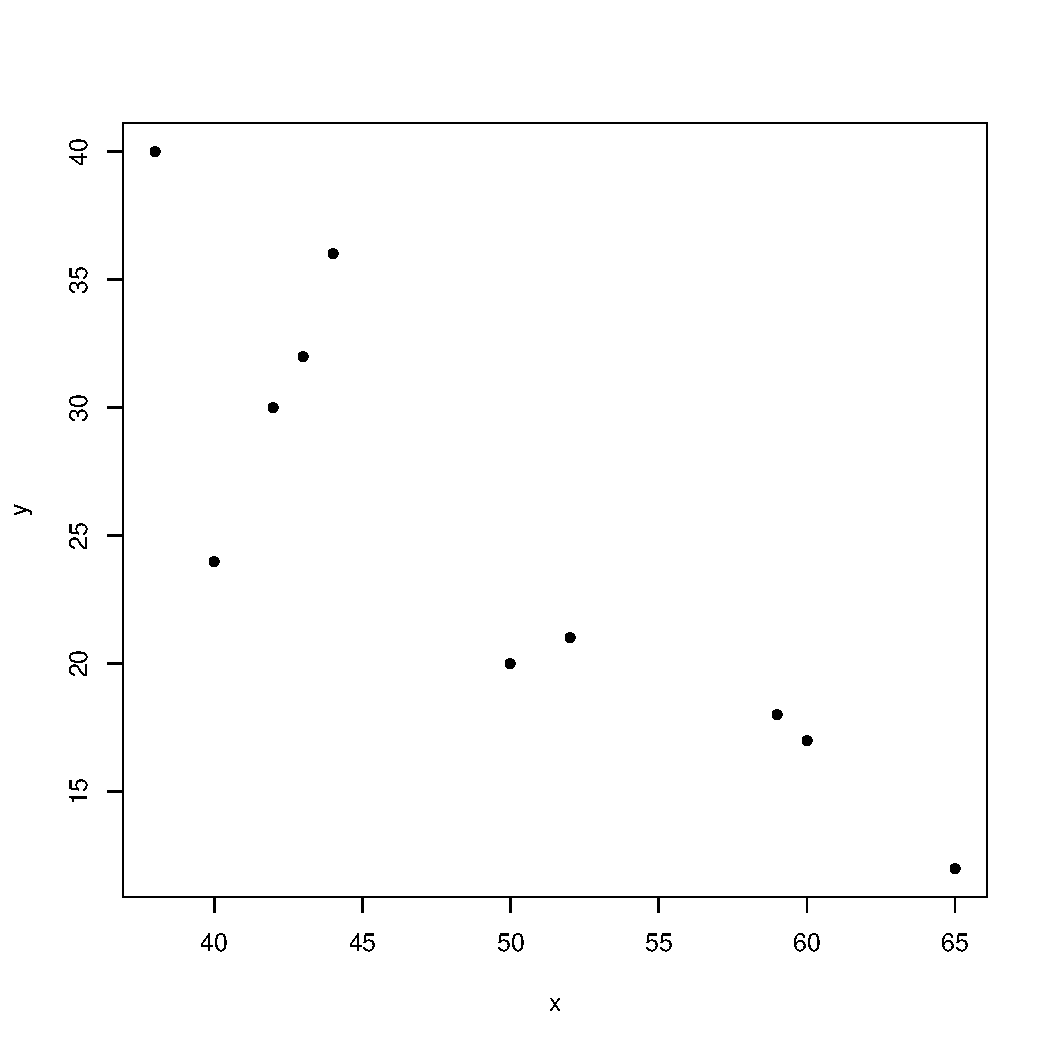
\includegraphics[width=\maxwidth]{figure/unnamed-chunk-3-1}

\end{knitrout}
        \caption{Relation entre les données de l'exercice
          \ref{chap:simple}.\ref{ex:simple:base}}
        \label{fig:simple:base}
      \end{figure}
    \item Les équations normales sont les équations à résoudre pour
      trouver les estimateurs de $\beta_0$ et $\beta_1$ minimisant la
      somme des carrés
      \begin{align*}
        S(\beta_0, \beta_1)
        &=\sum_{t = 1}^n \varepsilon^2_t \\
        &=\sum_{t = 1}^n \left(Y_t-\beta_0-\beta_1X_t\right)^2.
      \end{align*}
      Or,
      \begin{align*}
        \frac{\partial S}{\partial \beta_0}
        &= -2 \sum_{t=1}^n (Y_t - \beta_0 - \beta_1 X_t) \\
        \frac{\partial S}{\partial \beta_1}
        &= -2 \sum_{t=1}^n (Y_t - \beta_0 - \beta_1 X_t) X_t,
      \end{align*}
      d'où les équations normales sont
      \begin{align*}
        \sum_{t=1}^n (Y_t - \hat{\beta}_0 - \hat{\beta}_1 X_t) &= 0 \\
        \sum_{t=1}^n (Y_t - \hat{\beta}_0 - \hat{\beta}_1 X_t) X_t &= 0.
      \end{align*}
    \item Par la première des deux équations normales, on trouve
      \begin{displaymath}
        \sum_{t=1}^nY_t-n\hat{\beta}_0-\hat{\beta}_1\sum_{t=1}^nX_t = 0,
      \end{displaymath}
      soit, en isolant $\hat{\beta}_0$,
      \begin{displaymath}
        \hat{\beta}_0=\frac{\sum_{t=1}^nY_t-\hat{\beta}_1\sum_{t=1}^nX_t}{n}=\bar{Y}-\hat{\beta}_1\bar{X}.
      \end{displaymath}
      De la seconde équation normale, on obtient
      \begin{displaymath}
        \sum_{t=1}^n X_t Y_t -
        \hat{\beta}_0 \sum_{t=1}^n X_t -
        \hat{\beta}_1 \sum_{t=1}^n X_t^2 = 0
      \end{displaymath}
      puis, en remplaçant $\hat{\beta}_0$ par la valeur obtenue ci-dessus,
      \begin{displaymath}
        \hat{\beta}_1
        \left(
          \sum_{t=1}^n X_t^2 - n \bar{X}^2
        \right) =
        \sum_{t=1}^n X_t Y_t - n \bar{X} \bar{Y}.
      \end{displaymath}
      Par conséquent,
      \begin{align*}
        \hat{\beta}_1
        &= \frac{\sum_{t=1}^n X_t Y_t - n \bar{X}\bar{Y}}{\sum_{t=1}^n
          X_t^2 - n \bar{X}^2} \\
        &= \frac{\nombre{11654} - (10)(49,3)(25)}{\nombre{25103} -
          (10)(49,3)^2} \\
        &= -0,8407 \\
        \intertext{et}
        \hat{\beta}_0
        &=\bar{Y}-\hat{\beta}_1\bar{X}\\
        &=25 - (-0,8407)(49,3)\\
        &=66,4488.
      \end{align*}
    \item On peut calculer les prévisions correspondant à $X_1, \dots,
      X_{10}$ --- ou valeurs ajustées --- à partir de la relation
      $\hat{Y}_t = 66,4488 - 0,8407 X_t$, $t = 1, 2, \dots, 10$. Avec
      \textsf{R}, on crée un objet de type modèle de régression avec
      \texttt{lm} et on en extrait les valeurs ajustées avec
      \texttt{fitted}:
\begin{knitrout}
\definecolor{shadecolor}{rgb}{0.969, 0.969, 0.969}\color{fgcolor}\begin{kframe}
\begin{alltt}
\hlstd{fit} \hlkwb{<-} \hlkwd{lm}\hlstd{(y} \hlopt{~} \hlstd{x)}
\hlkwd{fitted}\hlstd{(fit)}
\end{alltt}
\begin{verbatim}
##        1        2        3        4        5        6
## 11.80028 30.29670 29.45596 16.84476 16.00401 24.41148
##        7        8        9       10
## 22.72998 34.50044 31.13745 32.81894
\end{verbatim}
\end{kframe}
\end{knitrout}
      Pour ajouter la droite de régression au graphique de la figure
      \ref{fig:simple:base}, il suffit d'utiliser la fonction
      \texttt{abline} avec en argument l'objet créé avec
      \texttt{lm}. L'ordonnée à l'origine et la pente de la droite
      seront extraites automatiquement. Voir la figure \ref{fig:simple:base2}.
      \begin{figure}
        \centering
\begin{knitrout}
\definecolor{shadecolor}{rgb}{0.969, 0.969, 0.969}\color{fgcolor}\begin{kframe}
\begin{alltt}
\hlkwd{abline}\hlstd{(fit)}
\end{alltt}
\end{kframe}
\end{knitrout}
\begin{knitrout}
\definecolor{shadecolor}{rgb}{0.969, 0.969, 0.969}\color{fgcolor}
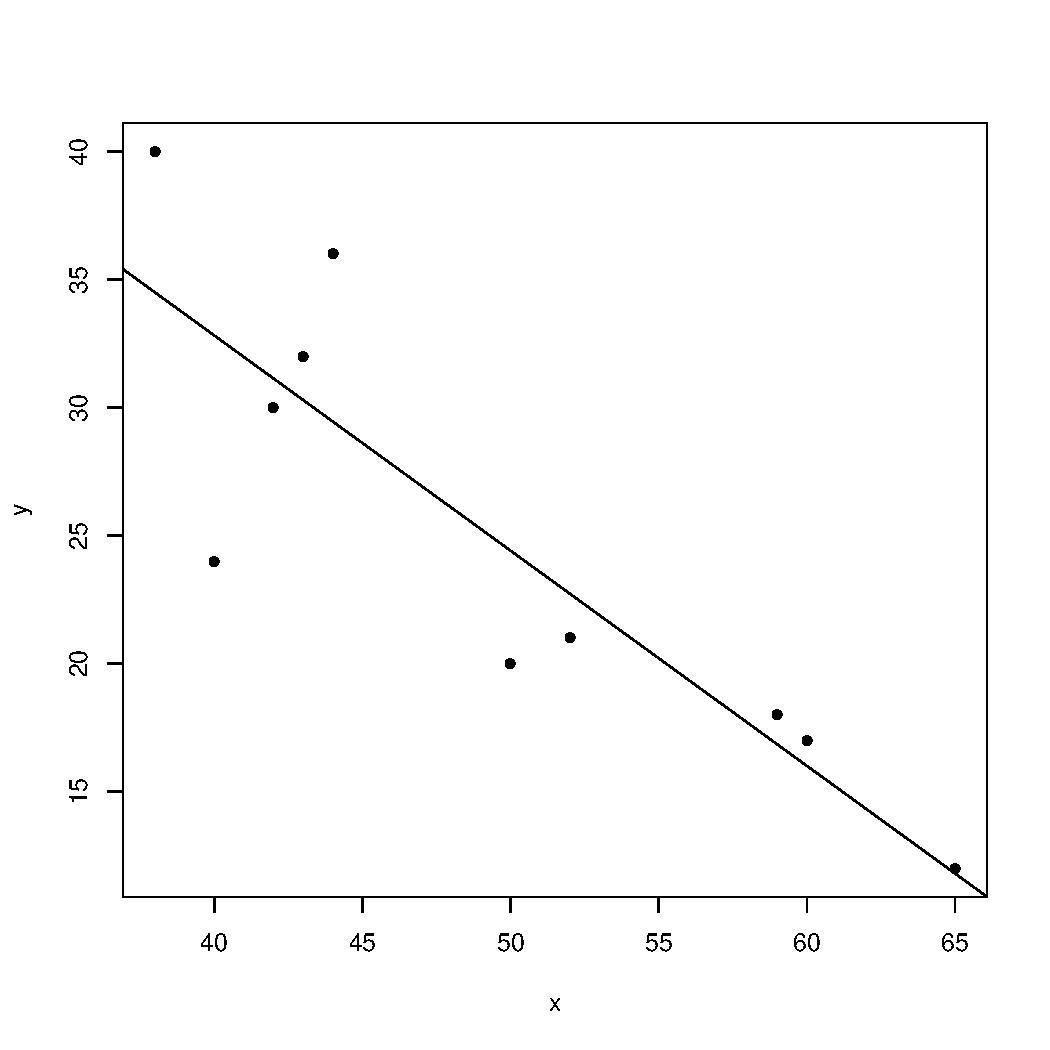
\includegraphics[width=\maxwidth]{figure/unnamed-chunk-6-1}

\end{knitrout}
        \caption{Relation entre les données de l'exercice
          \ref{chap:simple}.\ref{ex:simple:base} et la droite de
          régression}
        \label{fig:simple:base2}
      \end{figure}
    \item Les résidus de la régression sont $e_t = Y_t - \hat{Y}_t$,
      $t = 1, \dots, 10$. Dans \textsf{R}, la fonction
      \texttt{residuals} extrait les résidus du modèle:
\begin{knitrout}
\definecolor{shadecolor}{rgb}{0.969, 0.969, 0.969}\color{fgcolor}\begin{kframe}
\begin{alltt}
\hlkwd{residuals}\hlstd{(fit)}
\end{alltt}
\begin{verbatim}
##          1          2          3          4          5
##  0.1997243  1.7032953  6.5440421  1.1552437  0.9959905
##          6          7          8          9         10
## -4.4114773 -1.7299837  5.4995615 -1.1374514 -8.8189450
\end{verbatim}
\end{kframe}
\end{knitrout}
      On vérifie ensuite que la somme des résidus est
      (essentiellement) nulle:
\begin{knitrout}
\definecolor{shadecolor}{rgb}{0.969, 0.969, 0.969}\color{fgcolor}\begin{kframe}
\begin{alltt}
\hlkwd{sum}\hlstd{(}\hlkwd{residuals}\hlstd{(fit))}
\end{alltt}
\begin{verbatim}
## [1] -4.440892e-16
\end{verbatim}
\end{kframe}
\end{knitrout}
    \end{enumerate}
  
\end{solution}
\begin{solution}{2.2}
    \begin{enumerate}
    \item Nous avons le modèle de régression usuel. Les coefficients
      de la régression sont
      \begin{align*}
        \hat{\beta}_1
        &=\frac{\sum_{t=1}^8 X_tY_t-n\bar{X}\bar{Y}}{\sum_{t=1}^8
          X_t^2-n\bar{X}^2} \\
        &=\frac{146-(8)(32/8)(40/8)}{156-(8)(32/8)^2}  \\
        &=-0,5 \\
        \intertext{et}
        \hat{\beta}_0
        &=\bar{Y}-\hat{\beta}_1\bar{X} \\
        &=(40/8)-(-0,5)(32/8) \\
        &=7.
      \end{align*}
    \item Les sommes de carrés sont
      \begin{align*}
        \SST
        &=\sum_{t=1}^8(Y_t-\bar{Y})^2 \\
        &=\sum_{t=1}^8Y_t^2-n\bar{Y}^2 \\
        &=214-(8)(40/8)^2 \\
        &=14, \\
        \SSR
        &=\sum_{t=1}^8(\hat{Y}_t-\bar{Y})^2 \\
        &=\sum_{t=1}^8\hat{\beta}_1^2(X_t-\bar{X})^2 \\
        &=\hat{\beta}_1^2(\sum_{t=1}^8X_t^2-n\bar{X}^2) \\
        &=(-1/2)^2(156-(8)(32/8)^2) \\
        &=7.
      \end{align*}
      et $\SSE = \SST - \SSR = 14 - 7 = 7$. Par conséquent, $R^2 =
      SSR/SST = 7/14 = 0,5$, donc la régression explique 50~\% de la
      variation des $Y_t$ par rapport à leur moyenne $\bar{Y}$. Le
      tableau ANOVA est le suivant:
      \begin{center}
        \begin{tabular}{lcccc}
          \toprule
          Source & SS & d.l. & MS & Ratio F \\
          \midrule
          Régression & 7 & 1 & 7   & 6 \\
          Erreur     & 7 & 6 & 7/6 &  \\
          \midrule
          Total & 14 & 7 & & \\
          \bottomrule
        \end{tabular}
      \end{center}
    \end{enumerate}
  
\end{solution}
\begin{solution}{2.3}
    \begin{enumerate}
    \item Voir la figure \ref{fig:simple:women}.
      \begin{figure}
        \centering
\begin{knitrout}
\definecolor{shadecolor}{rgb}{0.969, 0.969, 0.969}\color{fgcolor}\begin{kframe}
\begin{alltt}
\hlkwd{data}\hlstd{(women)}
\hlkwd{plot}\hlstd{(weight} \hlopt{~} \hlstd{height,} \hlkwc{data} \hlstd{= women,} \hlkwc{pch} \hlstd{=} \hlnum{16}\hlstd{)}
\end{alltt}
\end{kframe}
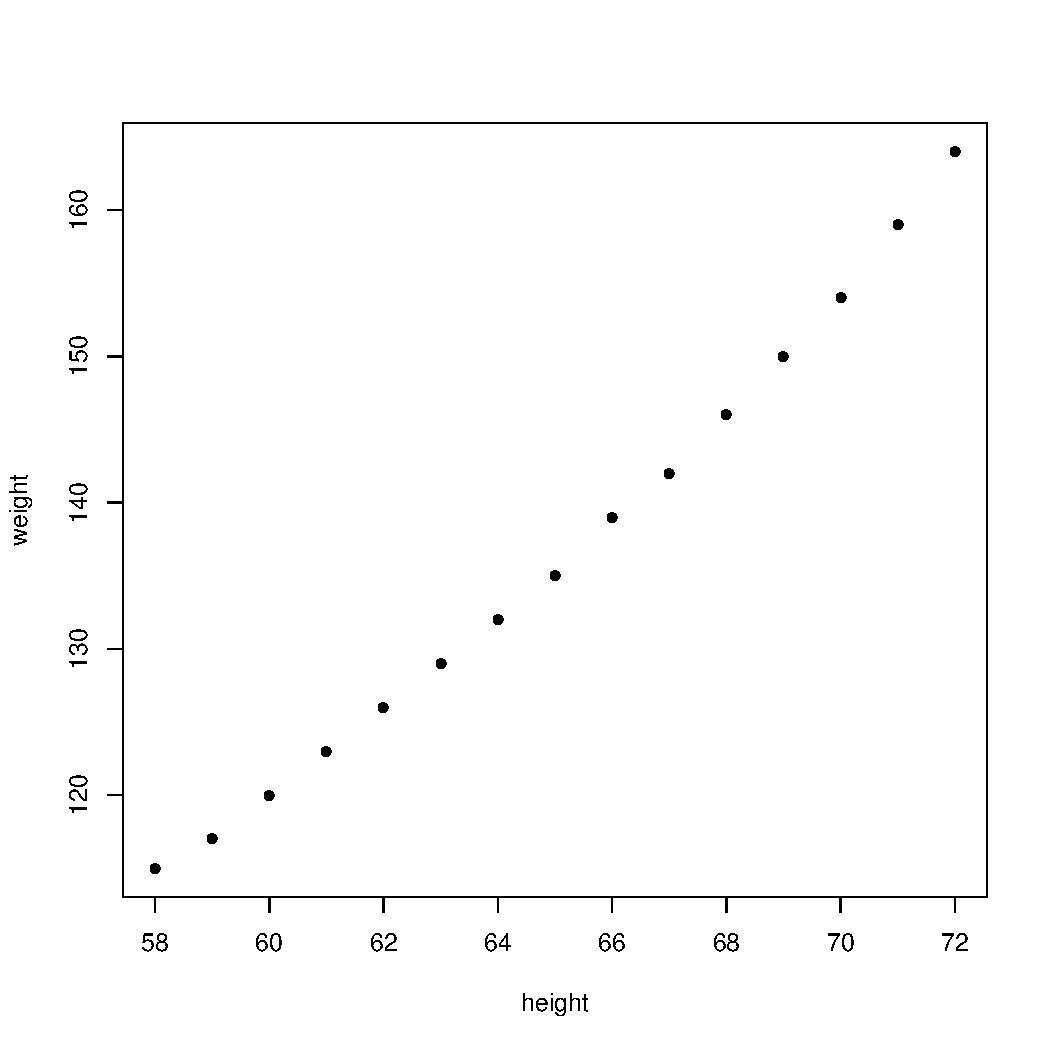
\includegraphics[width=\maxwidth]{figure/unnamed-chunk-10-1}

\end{knitrout}
        \caption{Relation entre la taille et le poids moyen de femmes américaines âgées de 30 à 39 ans (données \texttt{women})}
        \label{fig:simple:women}
      \end{figure}
    \item Le graphique montre qu'un modèle linéaire serait
      excellent. On estime les paramètres de ce modèle avec \texttt{lm}:
\begin{knitrout}
\definecolor{shadecolor}{rgb}{0.969, 0.969, 0.969}\color{fgcolor}\begin{kframe}
\begin{alltt}
\hlstd{(fit} \hlkwb{<-} \hlkwd{lm}\hlstd{(weight} \hlopt{~} \hlstd{height,} \hlkwc{data} \hlstd{= women))}
\end{alltt}
\begin{verbatim}
##
## Call:
## lm(formula = weight ~ height, data = women)
##
## Coefficients:
## (Intercept)       height
##      -87.52         3.45
\end{verbatim}
\end{kframe}
\end{knitrout}
    \item Voir la figure \ref{fig:simple:women2}.
      \begin{figure}
        \centering
\begin{knitrout}
\definecolor{shadecolor}{rgb}{0.969, 0.969, 0.969}\color{fgcolor}\begin{kframe}
\begin{alltt}
\hlkwd{abline}\hlstd{(fit)}
\end{alltt}
\end{kframe}
\end{knitrout}
\begin{knitrout}
\definecolor{shadecolor}{rgb}{0.969, 0.969, 0.969}\color{fgcolor}
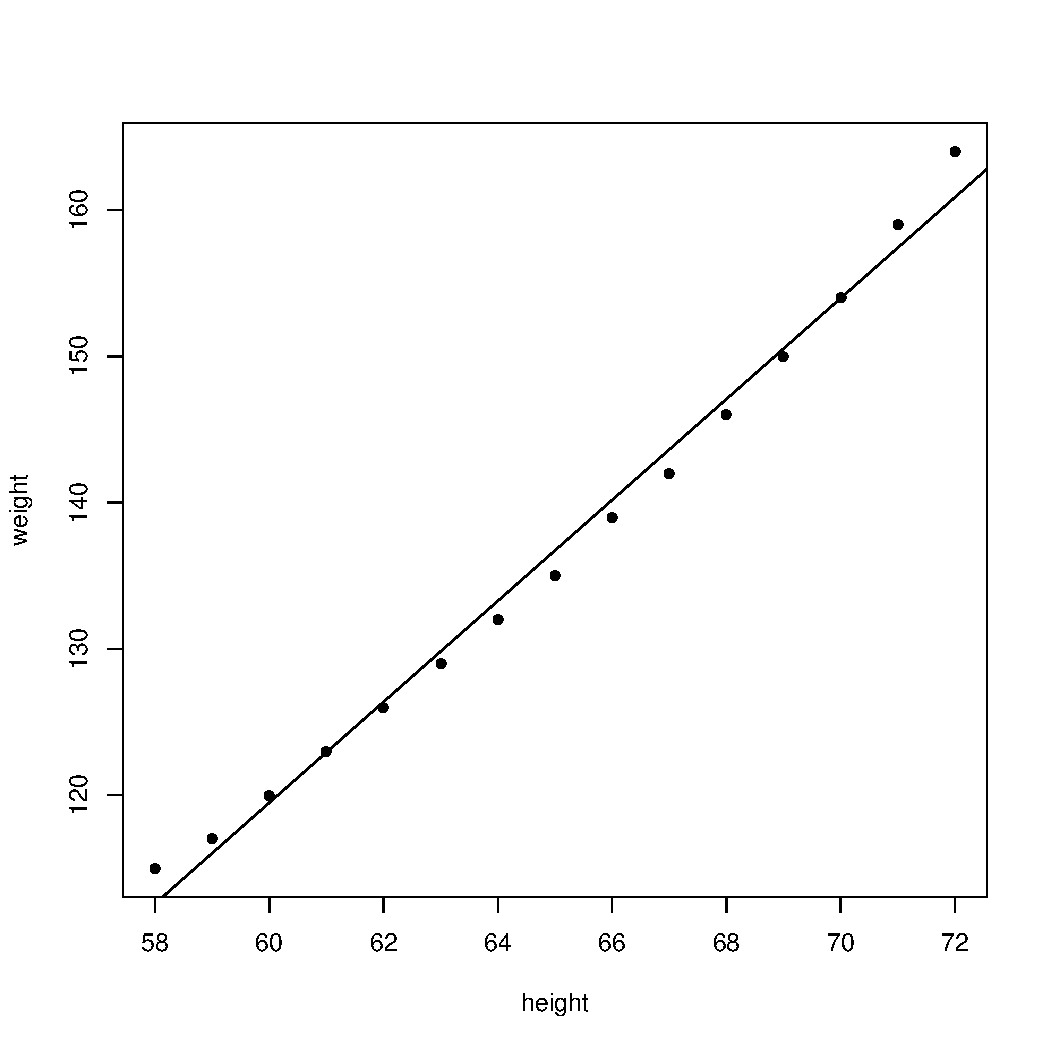
\includegraphics[width=\maxwidth]{figure/unnamed-chunk-13-1}

\end{knitrout}
        \caption{Relation entre les données \texttt{women} et droite de régression linéaire simple}
        \label{fig:simple:women2}
      \end{figure}
      On constate que l'ajustement est excellent.
    \item Le résultat de la fonction \texttt{summary} appliquée au
      modèle \texttt{fit} est le suivant:
\begin{knitrout}
\definecolor{shadecolor}{rgb}{0.969, 0.969, 0.969}\color{fgcolor}\begin{kframe}
\begin{alltt}
\hlkwd{summary}\hlstd{(fit)}
\end{alltt}
\begin{verbatim}
##
## Call:
## lm(formula = weight ~ height, data = women)
##
## Residuals:
##     Min      1Q  Median      3Q     Max
## -1.7333 -1.1333 -0.3833  0.7417  3.1167
##
## Coefficients:
##              Estimate Std. Error t value Pr(>|t|)
## (Intercept) -87.51667    5.93694  -14.74 1.71e-09 ***
## height        3.45000    0.09114   37.85 1.09e-14 ***
## ---
## Signif. codes:
## 0 '***' 0.001 '**' 0.01 '*' 0.05 '.' 0.1 ' ' 1
##
## Residual standard error: 1.525 on 13 degrees of freedom
## Multiple R-squared:  0.991,	Adjusted R-squared:  0.9903
## F-statistic:  1433 on 1 and 13 DF,  p-value: 1.091e-14
\end{verbatim}
\end{kframe}
\end{knitrout}
      Le coefficient de détermination est donc
      $R^2 = 0,991$, %$
      ce qui est près de 1 et confirme donc l'excellent
      ajustement du modèle évoqué en c).
    \item On a
\begin{knitrout}
\definecolor{shadecolor}{rgb}{0.969, 0.969, 0.969}\color{fgcolor}\begin{kframe}
\begin{alltt}
\hlkwd{attach}\hlstd{(women)}
\hlstd{SST} \hlkwb{<-} \hlkwd{sum}\hlstd{((weight} \hlopt{-} \hlkwd{mean}\hlstd{(weight))}\hlopt{^}\hlnum{2}\hlstd{)}
\hlstd{SSR} \hlkwb{<-} \hlkwd{sum}\hlstd{((}\hlkwd{fitted}\hlstd{(fit)} \hlopt{-} \hlkwd{mean}\hlstd{(weight))}\hlopt{^}\hlnum{2}\hlstd{)}
\hlstd{SSE} \hlkwb{<-} \hlkwd{sum}\hlstd{((weight} \hlopt{-} \hlkwd{fitted}\hlstd{(fit))}\hlopt{^}\hlnum{2}\hlstd{)}
\hlkwd{all.equal}\hlstd{(SST, SSR} \hlopt{+} \hlstd{SSE)}
\end{alltt}
\begin{verbatim}
## [1] TRUE
\end{verbatim}
\begin{alltt}
\hlkwd{all.equal}\hlstd{(}\hlkwd{summary}\hlstd{(fit)}\hlopt{$}\hlstd{r.squared, SSR}\hlopt{/}\hlstd{SST)}
\end{alltt}
\begin{verbatim}
## [1] TRUE
\end{verbatim}
\end{kframe}
\end{knitrout}
    \end{enumerate}
  
\end{solution}
\begin{solution}{2.4}
    Puisque $\hat{Y}_t = (\bar{Y} - \hat{\beta}_1 \bar{X}) +
    \hat{\beta}_1 X_t = \bar{Y} + \hat{\beta}_1 (X_t - \bar{X})$ et
    que $e_t = Y_t - \hat{Y}_t = (Y_t - \bar{Y}) - \hat{\beta}_1 (X_t
    - \bar{X})$, alors
    \begin{align*}
      \sum_{t = 1}^n (\hat{Y}_t - \bar{Y}) e_t
      &= \hat{\beta}_1
      \left(
        \sum_{t=1}^n (X_t - \bar{X})(Y_t - \bar{Y}) -
        \hat{\beta}_1 \sum_{t = 1}^n (X_t - \bar{X})^2
      \right) \\
      & = \hat{\beta}_1
      \left(
        S_{XY} - \frac{S_{XY}}{S_{XX}}\, S_{XX}
      \right) \\
      & = 0.
    \end{align*}
  
\end{solution}
\begin{solution}{2.5}
    On a un modèle de régression linéaire simple usuel avec $X_t =
    t$. Les estimateurs des moindres carrés des paramètres $\beta_0$ et
    $\beta_1$ sont donc
    \begin{align*}
      \hat{\beta}_0
      &= \bar{Y} - \hat{\beta}_1\, \frac{\sum_{t = 1}^n t}{n} \\
      \intertext{et}
      \hat{\beta}_1
      &= \frac{\sum_{t = 1}^n t Y_t - \bar{Y} \sum_{t = 1}^n t}{\sum_{t
          = 1}^n t^2 - n^{-1} (\sum_{t = 1}^n t)^2}.
    \end{align*}
    Or, puisque $\sum_{t = 1}^n t = n(n + 1)/2$ et $\sum_{t = 1}^n t^2
    = n(n + 1)(2n + 1)/6$, les expressions ci-dessus se simplifient en
    \begin{align*}
      \hat{\beta}_0
      & = \bar{Y} - \hat{\beta}_1\, \frac{n + 1}{2} \\
      \intertext{et}
      \hat{\beta}_1
      & = \frac{\sum_{t=1}^n t Y_t - n(n + 1) \bar{Y}/2}{n(n + 1)(2n +
        1)/6 - n(n + 1)^2/4} \\
      & = \frac{12 \sum_{t=1}^n t Y_t - 6 n (n + 1) \bar{Y}}{n (n^2 - 1)}.
    \end{align*}
  
\end{solution}
\begin{solution}{2.6}
    \begin{enumerate}
    \item L'estimateur des moindres carrés du paramètre $\beta$ est la
      valeur $\hat{\beta}$ minimisant la somme de carrés
      \begin{align*}
        S(\beta)
        &=\sum_{t = 1}^n \varepsilon_t^2 \\
        &=\sum_{t = 1}^n (Y_t - \beta X_t)^2.
      \end{align*}
      Or,
      \begin{displaymath}
        \frac{d}{d \beta}\, S(\beta) = -2 \sum_{t = 1}^n (Y_t -
        \hat{\beta} X_t) X_t,
      \end{displaymath}
      d'où l'unique équation normale de ce modèle est
      \begin{displaymath}
        \sum_{t = 1}^n X_t Y_t - \hat{\beta} \sum_{t=1}^n X_t^2 = 0.
      \end{displaymath}
      L'estimateur des moindres carrés de $\beta$ est donc
      \begin{displaymath}
        \hat{\beta} = \frac{\sum_{t=1}^n X_t Y_t}{\sum_{t=1}^n X_t^2}.
      \end{displaymath}
    \item On doit démontrer que $\esp{\hat{\beta}} = \beta$. On a
      \begin{align*}
        \esp{\hat{\beta}}
        &= \Esp{\frac{\sum_{t=1}^n X_t Y_t}{\sum_{t=1}^n X_t^2}} \\
        &= \frac{1}{\sum_{t=1}^n X_t^2} \sum_{t=1}^n X_t \esp{Y_t} \\
        &= \frac{1}{\sum_{t=1}^nX_t^2} \sum_{t=1}^n X_t \beta X_t \\
        &= \beta\, \frac{\sum_{t=1}^n X_t^2}{\sum_{t=1}^n X_t^2} \\
        &= \beta.
      \end{align*}
    \item Des hypothèses du modèle, on a
      \begin{align*}
        \var{\hat{\beta}}
        &= \Var{\frac{\sum_{t=1}^n X_t Y_t}{\sum_{t=1}^n X_t^2}} \\
        &= \frac{1}{(\sum_{t=1}^n X_t^2)^2} \sum_{t=1}^n X_t^2 \var{Y_t} \\
        &= \frac{\sigma^2}{(\sum_{t=1}^n X_t^2)^2} \sum_{t=1}^n X_t^2 \\
        &= \frac{\sigma^2}{\sum_{t=1}^n X_t^2}.
      \end{align*}
    \end{enumerate}
  
\end{solution}
\begin{solution}{2.7}
    On veut trouver les coefficients $c_1, \dots, c_n$ tels que
    $\esp{\beta^*} = \beta$ et $\var{\beta^*}$ est minimale. On
    cherche donc à minimiser la fonction
    \begin{align*}
      f(c_1, \dots, c_n)
      &= \var{\beta^*} \\
      &= \sum_{t=1}^n c_t^2 \var{Y_t} \\
      &= \sigma^2 \sum_{t=1}^n c_t^2
    \end{align*}
    sous la contrainte $\esp{\beta^*} = \sum_{t=1}^nc_t\esp{Y_t} =
    \sum_{t=1}^nc_t\beta X_t = \beta\sum_{t=1}^nc_tX_t = \beta$, soit
    $\sum_{t=1}^n c_t X_t = 1$ ou $g(c_1, \dots, c_n) = 0$ avec
    \begin{displaymath}
      g(c_1, \dots, c_n) = \sum_{t=1}^n c_t X_t - 1.
    \end{displaymath}
    Pour utiliser la méthode des multiplicateurs de Lagrange, on pose
    \begin{align*}
      \mathcal{L}(c_1, \dots, c_n,\lambda)
      &= f(c_1, \dots, c_n) - \lambda g(c_1, \dots, c_n), \\
      &= \sigma^2 \sum_{t=1}^n c_t^2 - \lambda
      \left(
        \sum_{t=1}^n c_t X_t - 1
      \right),
    \end{align*}
    puis on dérive la fonction $\mathcal{L}$ par rapport à chacune des
    variables $c_1, \dots, c_n$ et $\lambda$. On trouve alors
    \begin{align*}
      \frac{\partial \mathcal{L}}{\partial c_u}
      & = 2 \sigma^2 c_u - \lambda X_u, \quad u = 1, \dots, n \\
      \frac{\partial \mathcal{L}}{\partial \lambda}
      & = - \sum_{t=1}^n c_t X_t + 1.
    \end{align*}
    En posant les $n$ premières dérivées égales à zéro, on obtient
    \begin{displaymath}
      c_t = \frac{\lambda X_t}{2 \sigma^2}.
    \end{displaymath}
    Or, de la contrainte,
    \begin{displaymath}
      \sum_{t=1}^n c_t X_t =
      \frac{\lambda}{2\sigma^2} \sum_{t=1}^n X_t^2 = 1,
    \end{displaymath}
    d'où
    \begin{displaymath}
      \frac{\lambda}{2 \sigma^2} = \frac{1}{\sum_{t=1}^n X_t^2}
    \end{displaymath}
    et, donc,
    \begin{displaymath}
      c_t = \frac{X_t}{\sum_{t=1}^n X_t^2}.
    \end{displaymath}
    Finalement,
    \begin{align*}
      \beta^*
      & = \sum_{t=1}^n c_t Y_t \\
      & = \frac{\sum_{t=1}^n X_t Y_t}{\sum_{t=1}^n X_t^2} \\
      & = \hat{\beta}.
    \end{align*}
  
\end{solution}
\begin{solution}{2.8}
    \begin{enumerate}
    \item Tout d'abord, puisque $\MSE = \SSE/(n - 2) = \sum_{t=1}^n
      (Y_t - \hat{Y}_t)^2/(n - 2)$ et que $\esp{Y_t} =
      \esp{\hat{Y}_t}$, alors
      \begin{align*}
        \esp{MSE}
        &= \frac{1}{n - 2} \Esp{\sum_{t=1}^n (Y_t - \hat{Y}_t)^2} \\
        &= \frac{1}{n - 2} \sum_{t=1}^n \esp{(Y_t - \hat{Y}_t)^2} \\
        &= \frac{1}{n - 2} \sum_{t=1}^n \esp{((Y_t - \esp{Y_t}) -
          (\hat{Y}_t - \esp{\hat{Y}_t}))^2} \\
        &= \frac{1}{n - 2} \sum_{t=1}^n
        \left(
          \var{Y_t} + \var{\hat{Y}_t} - 2\, \Cov(Y_t, \hat{Y}_t)
        \right).
      \end{align*}
      Or, on a par hypothèse du modèle que $\Cov(Y_t, Y_s) =
      \Cov(\varepsilon_t, \varepsilon_s) = \delta_{ts} \sigma^2$, d'où
      $\var{Y_t} = \sigma^2$ et $\var{\bar{Y}} = \sigma^2/n$. D'autre
      part,
      \begin{align*}
        \var{\hat{Y}_t}
        &= \var{\bar{Y} + \hat{\beta}_1 (X_t - \bar{X})} \\
        &= \var{\bar{Y}} + (X_t - \bar{X})^2 \var{\hat{\beta}_1} +
        2 (X_t - \bar{X}) \Cov(\bar{Y}, \hat{\beta}_1)
      \end{align*}
      et l'on sait que
      \begin{align*}
        \var{\hat{\beta}_1}
        &= \frac{\sigma^2}{\sum_{t=1}^n(X_t-\bar{X})^2} \\
        \intertext{et que}
        \Cov(\bar{Y}, \hat{\beta}_1)
        & = \Cov
        \left(
          \frac{\sum_{t = 1}^n Y_t}{n},
          \frac{\sum_{s = 1}^n (X_s - \bar{X}) Y_s}{\sum_{t = 1}^n
            (X_t - \bar{X})^2}
        \right) \\
        &= \frac{1}{n \sum_{t = 1}^n (X_t - \bar{X})^2}
        \sum_{t = 1}^n \sum_{s = 1}^n \Cov(Y_t, (X_s - \bar{X}) Y_s) \\
        &= \frac{1}{n \sum_{t = 1}^n (X_t - \bar{X})^2}
        \sum_{t = 1}^n (X_s - \bar{X}) \var{Y_t} \\
        & = \frac{\sigma^2}{n \sum_{t = 1}^n (X_t - \bar{X})^2}
        \sum_{t = 1}^n (X_t - \bar{X}) \\
        & = 0,
      \end{align*}
      puisque $\sum_{i=1}^n(X_i - \bar{X}) = 0$. Ainsi,
      \begin{displaymath}
        \var{\hat{Y}_t} = \frac{\sigma^2}{n} +
        \frac{(X_t - \bar{X})^2 \sigma^2}{\sum_{t=1}^n (X_t - \bar{X})^2}.
      \end{displaymath}
      De manière similaire, on détermine que
      \begin{align*}
        \Cov(Y_t, \hat{Y}_t)
        &= \Cov(Y_t, \bar{Y} + \hat{\beta}_1 (X_t - \bar{X})) \\
        &= \Cov(Y_t, \bar{Y}) +
        (X_t - \bar{X}) \Cov(Y_t, \hat{\beta}_1) \\
        &= \frac{\sigma^2}{n} + \frac{(X_t -
          \bar{X})^2 \sigma^2}{\sum_{t=1}^n (X_t - \bar{X})^2}.
      \end{align*}
      Par conséquent,
      \begin{align*}
        \esp{(Y_t - \hat{Y}_t)^2}
        &= \frac{n - 1}{n}\, \sigma^2 -
        \frac{(X_t - \bar{X})^2 \sigma^2}{\sum_{t = 1}^n (X_t - \bar{X})^2} \\
        \intertext{et}
        \sum_{t=1}^n \esp{(Y_t - \hat{Y}_t)^2}
        & = (n - 2) \sigma^2,
      \end{align*}
      d'où $\esp{\MSE} = \sigma^2$.
    \item On a
      \begin{align*}
        \esp{\MSR}
        &= \esp{\SSR} \\
        &= \Esp{\sum_{t=1}^n (\hat{Y}_t - \bar{Y})^2} \\
        &= \sum_{t=1}^n \esp{\hat{\beta}_1^2 (X_t - \bar{X})^2} \\
        &= \sum_{t=1}^n (X_t - \bar{X})^2 \esp{\hat{\beta}_1^2} \\
        &= \sum_{t=1}^n (X_t - \bar{X})^2 (\var{\hat{\beta}_1} +
        \esp{\hat{\beta}_1}^2) \\
        &= \sum_{t=1}^n (X_t - \bar{X})^2
        \left(
          \frac{\sigma^2}{\sum_{t=1}^n (X_t - \bar{X})^2} + \beta_1^2
        \right) \\
        &= \sigma^2 + \beta_1^2 \sum_{t=1}^n (X_t - \bar{X})^2.
      \end{align*}
    \end{enumerate}
  
\end{solution}
\begin{solution}{2.9}
    \begin{enumerate}
    \item Il faut exprimer $\hat{\beta}_0^\prime$ et
      $\hat{\beta}_1^\prime$ en fonction de $\hat{\beta}_0$ et
      $\hat{\beta}_1$. Pour ce faire, on trouve d'abord une expression
      pour chacun des éléments qui entrent dans la définition de
      $\hat{\beta}_1^\prime$. Tout d'abord,
      \begin{align*}
        \bar{X}^\prime
        &= \frac{1}{n} \sum_{t=1}^n X_t^\prime \\
        &= \frac{1}{n} \sum_{t=1}^n (c + d X_t) \\
        &= c + d \bar{X},
      \end{align*}
      et, de manière similaire, $\bar{Y}^\prime = a + b \bar{Y}$. Ensuite,
      \begin{align*}
        S_{XX}^\prime
        &= \sum_{t=1}^n (X_t^\prime - \bar{X}^\prime)^2 \\
        &= \sum_{t=1}^n (c + d X_t - c - d \bar{X})^2 \\
        &= d^2 S_{XX}
      \end{align*}
      et $S_{YY}^\prime = b^2 S_{YY}$, $S_{XY}^\prime = bd S_{XY}$.
      Par conséquent,
      \begin{align*}
        \hat{\beta}_1^\prime
        &= \frac{S_{XY}^\prime}{S_{XX}^\prime} \\
        &= \frac{bd S_{XY}}{d^2 S_{XX}} \\
        &= \frac{b}{d}\, \hat{\beta}_1 \\
        \intertext{et}
        \hat{\beta}_0^\prime
        &= \bar{Y}^\prime - \hat{\beta}_1^\prime \bar{X}^\prime \\
        &= a + b \bar{Y} - \frac{b}{d}\, \hat{\beta}_1 (c + d \bar{X}) \\
        &= a - \frac{bc}{d}\, \hat{\beta}_1 + b (\bar{Y} -
        \hat{\beta}_1 \bar{X}) \\
        &= a - \frac{bc}{d}\, \hat{\beta}_1 + b \hat{\beta}_0.
      \end{align*}
    \item Tout d'abord, on établit que
      \begin{align*}
        R^2
        &= \frac{\SSR}{\SST} \\
        &= \frac{\sum_{t=1}^n (\hat{Y_t} - \bar{Y})^2}{\sum_{t=1}^n
          (Y_t - \bar{Y})^2} \\
        &= \hat{\beta}_1^2\, \frac{\sum_{t=1}^n (X_t -
          \bar{X})^2}{\sum_{t=1}^n (Y_t - \bar{Y})^2} \\
        &= \hat{\beta}_1^2\, \frac{S_{XX}}{S_{YY}}.
      \end{align*}
      Maintenant, avec les résultats obtenus en a), on démontre
      directement que
      \begin{align*}
        (R^2)^\prime
        &= (\hat{\beta}_1^\prime)^2 \frac{S_{XX}^\prime}{S_{YY}^\prime} \\
        &=
        \left(
          \frac{b}{d}
        \right)^2\,
        \hat{\beta}_1^2\, \frac{d^2 S_{XX}}{b^2 S_{YY}} \\
        &= \hat{\beta}_1^2\, \frac{S_{XX}}{S_{YY}} \\
        &= R^2.
      \end{align*}
    \end{enumerate}
  
\end{solution}
\begin{solution}{2.10}
    Considérons un modèle de régression usuel avec l'ensemble de
    données $(X_1, Y_1), \dots, (X_n, Y_n), (m \bar{X}, m \bar{Y})$,
    où $\bar{X} = n^{-1} \sum_{t = 1}^n X_t$, $\bar{Y} = n^{-1}
    \sum_{t = 1}^n Y_t$, $m = n/a$ et $a = \sqrt{n + 1} - 1$. On
    définit
    \begin{align*}
      \bar{X}^\prime
      &= \frac{1}{n + 1} \sum_{t = 1}^{n + 1} X_t \\
      &= \frac{1}{n + 1} \sum_{t = 1}^n X_t + \frac{m}{n + 1} \bar{X} \\
      &= k \bar{X} \\
      \intertext{et, de manière similaire,}
      \bar{Y}^\prime
      &= k \bar{Y},
      \intertext{où}
      k
      &= \frac{n + m}{n + 1} \\
      &= \frac{n (a + 1)}{a (n + 1)}.
    \end{align*}
    L'expression pour l'estimateur des moindres carrés de la pente de
    la droite de régression pour cet ensemble de données est
    \begin{align*}
      \hat{\beta}_1
      &= \frac{\sum_{t = 1}^{n + 1} X_t Y_t - (n + 1)
        \bar{X}^\prime \bar{Y}^\prime}{%
        \sum_{t = 1}^{n + 1} X_t^2 - (n + 1) (\bar{X}^\prime)^2} \\
      &= \frac{\sum_{t = 1}^n X_t Y_t + m^2 \bar{X} \bar{Y} - (n + 1)
        k^2 \bar{X} \bar{Y}}{%
        \sum_{t = 1}^n X_t^2 + m^2 \bar{X}^2 - (n + 1) k^2 \bar{X}^2}.
    \end{align*}
    Or,
    \begin{align*}
      m^2 - k^2 (n + 1)
      &= \frac{n^2}{a^2} - \frac{n^2 (a + 1)^2}{a^2 (n + 1)} \\
      &= \frac{n^2 (n + 1) - n^2 (n + 1)}{a^2 (n + 1)} \\
      &= 0.
    \end{align*}
    Par conséquent,
    \begin{align*}
      \hat{\beta}_1
      &= \frac{\sum_{t = 1}^n X_t Y_t}{\sum_{t = 1}^n X_t^2} \\
      &= \hat{\beta}.
    \end{align*}
    Interprétation: en ajoutant un point bien spécifique à n'importe
    quel ensemble de données, on peut s'assurer que la pente de la
    droite de régression sera la même que celle d'un modèle passant
    par l'origine. Voir la figure \ref{fig:simple:pointmagique} pour
    une illustration du phénomène.

    \begin{figure}
      \centering
\begin{knitrout}
\definecolor{shadecolor}{rgb}{0.969, 0.969, 0.969}\color{fgcolor}
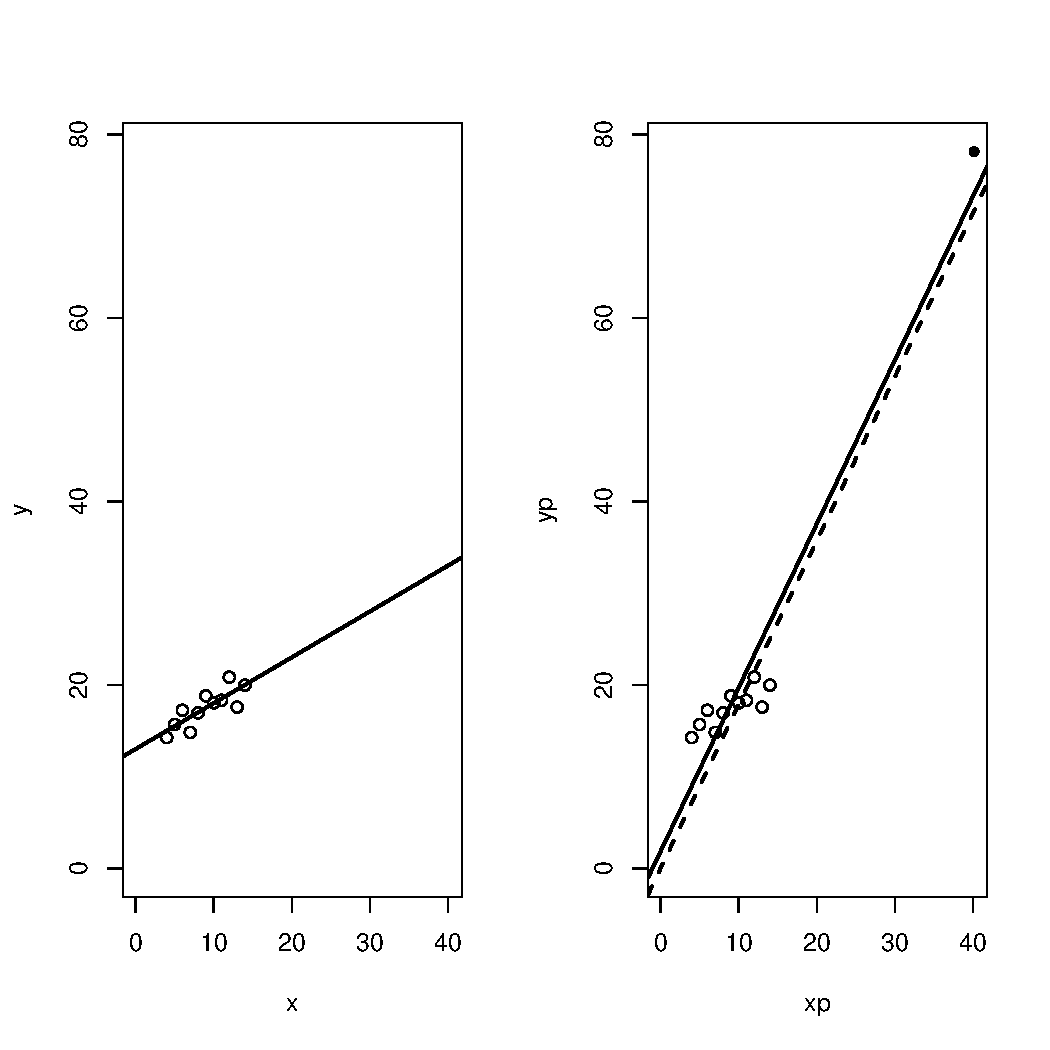
\includegraphics[width=\maxwidth]{figure/unnamed-chunk-17-1}

\end{knitrout}
      \caption{Illustration de l'effet de l'ajout d'un point spécial à
        un ensemble de données. À gauche, la droite de régression
        usuelle. À droite, le même ensemble de points avec le point
        spécial ajouté (cercle plein), la droite de régression avec ce
        nouveau point (ligne pleine) et la droite de régression
        passant par l'origine (ligne pointillée). Les deux droites
        sont parallèles.}
      \label{fig:simple:pointmagique}
    \end{figure}
  
\end{solution}
\begin{solution}{2.11}
    Puisque, selon le modèle, $\varepsilon_t \sim N(0, \sigma^2)$ et
    que $Y_t = \beta_0 + \beta_1 X_t + \varepsilon_t$, alors $Y_t \sim
    N(\beta_0 + \beta_1 X_t, \sigma^2)$. De plus, on sait que
    \begin{align*}
      \hat{\beta}_1
      &= \frac{\sum_{t=1}^n (X_t - \bar{X})(Y_t - \bar{Y})}{%
        \sum_{t=1}^n (X_t - \bar{X})^2} \\
      &= \frac{\sum_{t=1}^n (X_t - \bar{X}) Y_t}{%
        \sum_{t=1}^n (X_t - \bar{X})^2},
    \end{align*}
    donc l'estimateur $\hat{\beta}_1$ est une combinaison linéaire des
    variables aléatoires $Y_1, \dots, Y_n$. Par conséquent,
    $\hat{\beta}_1 \sim N(\esp{\hat{\beta}_1}, \var{\hat{\beta}_1})$,
    où $\esp{\hat{\beta}_1} = \beta_1$ et $\var{\hat{\beta}_1} =
    \sigma^2/S_{XX}$ et, donc,
    \begin{displaymath}
      \Pr
      \left[
        -z_{\alpha/2} <
        \frac{\hat{\beta}_1 - \beta_1}{\sigma/\sqrt{S_{XX}}} <
        z_{\alpha/2}
      \right] = 1 - \alpha.
    \end{displaymath}
    Un intervalle de confiance de niveau $1 - \alpha$ pour le
    paramètre $\beta_1$ lorsque la variance $\sigma^2$ est connue est donc
    \begin{displaymath}
      \beta_1 \in \hat{\beta}_1 \pm z_{\alpha/2}
      \frac{\sigma}{\sqrt{\sum_{t=1}^n (X_t - \bar{X})^2}}.
    \end{displaymath}
  
\end{solution}
\begin{solution}{2.12}
    L'intervalle de confiance pour $\beta_1$ est
    \begin{align*}
      \beta_1
      &\in \hat{\beta}_1 \pm t_{\alpha/2}(n - 2)
      \sqrt{\frac{\hat{\sigma}^2}{S_{XX}}} \\
      &\in \hat{\beta}_1 \pm t_{0,025}(20 - 2) \sqrt{\frac{MSE}{S_{XX}}}.
     \end{align*}
     On nous donne $\SST = S_{YY} = \nombre{20838}$ et $S_{XX} =
     \nombre{10668}$. Par conséquent,
     \begin{align*}
       \SSR
       &= \hat{\beta}_1^2 \sum_{t=1}^{20} (X_t - \bar{X})^2 \\
       &= (-1,104)^2(\nombre{10668}) \\
       &= \nombre{13002,33} \\
       \SSE
       &= \SST - \SSR \\
       &= \nombre{7835,67} \\
       \intertext{et}
       \MSE
       &= \frac{\SSE}{18} \\
       &= 435,315.
     \end{align*}
     De plus, on trouve dans une table de quantiles de la loi de
     Student (ou à l'aide de la fonction \texttt{qt} dans \textsf{R})
     que $t_{0,025}(18) = 2,101$. L'intervalle de confiance recherché
     est donc
     \begin{align*}
       \beta_1
       &\in -1,104 \pm 2,101 \sqrt{\frac{435,315}{\nombre{10668}}} \\
       &\in (-1,528, -0,680).
     \end{align*}
  
\end{solution}
\begin{solution}{2.13}
    \begin{enumerate}
    \item On trouve aisément les estimateurs de la pente et de
      l'ordonnée à l'origine de la droite de régression:
      \begin{align*}
        \hat{\beta}_1
        &= \frac{\sum_{t=1}^n X_t Y_t - n \bar{X}\bar{Y}}{%
          \sum_{t=1}^n X_t^2 - n \bar{X}^2} \\
        &= 1,436 \\
        \hat{\beta}_0
        &= \bar{Y} - \hat{\beta}_1 \bar{X} \\
        &= 9,273.
      \end{align*}
    \item Les sommes de carrés sont
      \begin{align*}
        \SST
        &= \sum_{t=1}^n Y_t^2 - n \bar{Y}^2 \\
        &= 1194 - 11 (9,273)^2 \\
        &= 248,18 \\
        \SSR
        &= \hat{\beta}_1^2
        \left(
          \sum_{t=1}^n X_t^2 - n \bar{X}^2
        \right) \\
        &= (1,436)^2 (110 - 11 (0)) \\
        &= 226,95
      \end{align*}
      et $\SSE = \SST - \SSR = 21,23$. Le tableau d'analyse de
      variance est donc le suivant:

      \begin{center}
        \begin{tabular}{lrrrc}
          \toprule
          Source
          & \multicolumn{1}{c}{SS}
          & \multicolumn{1}{c}{d.l.}
          & \multicolumn{1}{c}{MS}
          & Ratio F \\
          \midrule
          Régression & 226,95 &   1  & 226,95 & 96,21 \\
          Erreur     &  21,23 &   9  &   2,36 &  \\
          \midrule
          Total      & 248,18 &  10  &        & \\
          \bottomrule
        \end{tabular}
      \end{center}

      Or, puisque $t = \sqrt{F} = 9,809 > t_{\alpha/2}(n-2) =
      t_{0,025}(9) = 2,26$, on rejette l'hypothèse $H_0: \beta_1 =
      0$ soit, autrement dit, la pente est significativement
      différente de zéro.
    \item Puisque la variance $\sigma^2$ est inconnue, on l'estime par
      $s^2 = \MSE = 2,36$. On a alors
      \begin{align*}
        \beta_1
        &\in \hat{\beta}_1 \pm t_{\alpha/2}(n-2)
        \sqrt{\widehat{\mathrm{Var}}[\hat{\beta}_1]} \\
        &\in 1,436 \pm 2,26 \sqrt{\frac{2,36}{110}} \\
        &\in (1,105, 1,768).
      \end{align*}
    \item Le coefficient de détermination de la régression est $R^2 =
      \SSR/\SST = 226,95/248,18 = 0,914$, ce qui indique que
      l'ajustement du modèle aux données est très bon. En outre, suite
      au test effectué à la partie b), on conclut que la régression
      est globalement significative.  Toutes ces informations portent
      à conclure qu'il n'y a pas lieu d'utiliser un autre modèle.
    \end{enumerate}
  
\end{solution}
\begin{solution}{2.14}
    On doit déterminer si la régression est significative, ce qui peut
    se faire à l'aide de la statistique $F$. Or, à partir de
    l'information donnée dans l'énoncé, on peut calculer
    \begin{align*}
      \hat{\beta}_1
      &= \frac{\sum_{t=1}^{50} X_t Y_t - 50 \bar{X} \bar{Y}}{%
        \sum_{t=1}^{50} X_t^2 - 50 \bar{X})^2} \\
      &= -0,0110 \\
      \SST
      &= \sum_{t=1}^{50} Y_t^2 - 50 \bar{Y}^2 \\
      &= 78,4098 \\
      \SSR
      &= \hat{\beta}_1^2 \sum_{t=1}^{50} (X_t - \bar{X})^2 \\
      &= 1,1804 \\
      \SSE
      &= \SST - \SSR \\
      &= 77,2294 \\
      \intertext{d'où}
      \MSR
      &= 1,1804 \\
      \MSE
      &= \frac{\SSE}{50 - 2} \\
      &= 1,6089 \\
      \intertext{et, enfin,}
      F
      &= \frac{\MSR}{\MSE} \\
      &= 0,7337.
    \end{align*}
    Soit $F$ une variable aléatoire ayant une distribution de Fisher
    avec 1 et 48 degrés de liberté, soit la même distribution que la
    statistique $F$ sous l'hypothèse $H_0: \beta_1 = 0$. On a que
    $\Pr[F > 0,7337] = 0,3959$, donc la valeur $p$ du test $H_0:
    \beta_1 = 0$ est $0,3959$. Une telle valeur $p$ est généralement
    considérée trop élevée pour rejeter l'hypothèse $H_0$. On ne peut
    donc considérer la relation entre la ligne de vie et l'espérance
    de vie comme significative. (Ou on ne la considère significative
    qu'avec un niveau de confiance de $1 - p = 60,41$~\%.)
  
\end{solution}
\begin{solution}{2.15}
    Premièrement, selon le modèle de régression passant par l'origine,
    $Y_0 = \beta X_0 + \varepsilon_0$ et $\hat{Y}_0 = \hat{\beta}
    X_0$. Considérons, pour la suite, la variable aléatoire $Y_0 -
    \hat{Y}_0$. On voit facilement que $\esp{\hat{\beta}} = \beta$,
    d'où $\esp{Y_0 - \hat{Y}_0} = \esp{\beta X_0 + \varepsilon_0 -
      \hat{\beta} X_0} = \beta X_0 - \beta X_0 = 0$ et
    \begin{displaymath}
      \var{Y_0 - \hat{Y}_0} = \var{Y_0} + \var{\hat{Y}_0} - 2\,
      \Cov(Y_0, \hat{Y}_0).
    \end{displaymath}
    Or, $\Cov(Y_0, \hat{Y}_0) = 0$ par l'hypothèse ii) de l'énoncé,
    $\var{Y_0} = \sigma^2$ et $\var{\hat{Y}_0} = X_0^2\,
    \var{\hat{\beta}}$. De plus,
    \begin{align*}
      \var{\hat{\beta}}
      &= \frac{1}{(\sum_{t=1}^n X_t^2)^2} \sum_{t=1}^n X_t^2\,
      \var{Y_t} \\
      &= \frac{\sigma^2}{\sum_{t=1}^n X_t^2}
    \end{align*}
    d'où, finalement,
    \begin{displaymath}
      \var{Y_0 - \hat{Y}_0} =
      \sigma^2 \left( 1 + \frac{X_0^2}{\sum_{t=1}^n X_t^2} \right).
    \end{displaymath}
    Par l'hypothèse de normalité et puisque $\hat{\beta}$ est une
    combinaison linéaire de variables aléatoires normales,
    \begin{displaymath}
      Y_0 - \hat{Y}_0 \sim N
      \left(
        0, \sigma^2 \left( 1 + \frac{X_0^2}{\sum_{t=1}^n X_t^2} \right)
      \right)
    \end{displaymath}
    ou, de manière équivalente,
    \begin{displaymath}
      \frac{Y_0 - \hat{Y}_0}{\sigma \sqrt{1 + X_0^2/\sum_{t=1}^n X_t^2}}
      \sim N(0, 1).
    \end{displaymath}
    Lorsque la variance $\sigma^2$ est estimée par $s^2$, alors
    \begin{displaymath}
      \frac{Y_0 - \hat{Y}_0}{s \sqrt{1 + X_0^2/\sum_{t=1}^n X_t^2}}
      \sim t(n - 1).
    \end{displaymath}
    La loi de Student a $n - 1$ degrés de liberté puisque le modèle
    passant par l'origine ne compte qu'un seul paramètre. Les bornes
    de l'intervalle de confiance pour la vraie valeur de $Y_0$ sont
    donc
    \begin{displaymath}
      \hat{Y}_0 \pm t_{\alpha/2}(n - 1)\, s\, \sqrt{1 +
        \frac{X_0^2}{\sum_{t=1}^n X_t^2}}.
    \end{displaymath}
  
\end{solution}
\begin{solution}{2.16}
    \begin{enumerate}
    \item Soit $X_1, \dots, X_{10}$ les valeurs de la masse monétaire
      et $Y_1, \dots, Y_{10}$ celles du PNB. On a $\bar{X} = 3,72$,
      $\bar{Y} = 7,55$, $\sum_{t = 1}^{10} X_t^2 = 147,18$, $\sum_{t =
        1}^{10} Y_t^2 = 597,03$ et $\sum_{t = 1}^{10} X_t Y_t =
      295,95$. Par conséquent,
      \begin{align*}
        \hat{\beta}_1
        &= \frac{\sum_{t=1}^{10} X_t Y_t - 10 \bar{X} \bar{Y}}{%
          \sum_{t=1}^{10} X_t^2 - 10 \bar{X}^2} \\
        &= 1,716 \\
        \intertext{et}
        \hat{\beta}_0
        &= \bar{Y} - \hat{\beta}_1 \bar{X} \\
        &= 1,168.
      \end{align*}
      On a donc la relation linéaire $\text{PNB} = 1,168 + 1,716
      \text{ MM}$.
    \item Tout d'abord, on doit calculer l'estimateur $s^2$ de la
      variance car cette quantité entre dans le calcul des intervalles
      de confiance demandés. Pour les calculs à la main, on peut
      éviter de calculer les valeurs de $\hat{Y}_1, \dots,
      \hat{Y}_{10}$ en procédant ainsi:
      \begin{align*}
        \SST
        &= \sum_{t=1}^{10} Y_t^2 - 10 \bar{Y}^2 \\
        &= 27,005 \\
        \SSR
        &= \hat{\beta}_1^2
        \left(
          \sum_{t=1}^{10} X_t^2 - 10 \bar{X}^2
        \right) \\
        &= 25,901,
      \end{align*}
      puis $\SSE = \SST - \SSR = 1,104$ et $s^2 = \MSE = \SSE/(10 - 2)
      = 0,1380$.  On peut maintenant construire les intervalles de
      confiance:
      \begin{align*}
        \beta_0
        &\in \hat{\beta}_0 \pm t_{\alpha/2}(n - 2)\, s\,
        \sqrt{\frac{1}{n} + \frac{\bar{X}^2}{S_{XX}}} \\
        &\in 1,168 \pm (2,306) (0,3715)
        \sqrt{\frac{1}{10} + \frac{3,72^2}{8,796}} \\
        &\in (0,060, 2,276) \\
        \beta_1
        &\in \hat{\beta}_1 \pm t_{\alpha/2}(n - 2)\, s\,
        \sqrt{\frac{1}{S_{XX}}} \\
        &\in 1,716 \pm (2,306) (0,3715) \sqrt{\frac{1}{8,796}} \\
        &\in (1,427, 2,005).
      \end{align*}
      Puisque l'intervalle de confiance pour la pente $\beta_1$ ne
      contient ni la valeur 0, ni la valeur 1, on peut rejeter, avec
      un niveau de confiance de 95~\%, les hypothèses $H_0: \beta_1 =
      0$ et $H_0: \beta_1 = 1$.
    \item Par l'équation obtenue en a) liant le PNB à la masse
      monétaire (MM), un PNB de 12,0 correspond à une masse monétaire
      de
      \begin{align*}
        \text{MM}
        &= \frac{12,0 - 1,168}{1,716} \\
        &= 6,31.
      \end{align*}
    \item On cherche un intervalle de confiance pour la droite de
      régression en $\text{MM}_{1997} = 6,31$ ainsi qu'un intervalle
      de confiance pour la prévision $\text{PNB} = 12,0$ associée à
      cette même valeur de la masse monétaire.  Avec une probabilité
      de $\alpha = 95~\%$, le PNB moyen se trouve dans l'intervalle
      \begin{displaymath}
        12,0 \pm t_{\alpha/2}(n - 2)\, s\,
        \sqrt{\frac{1}{n} + \frac{(6,31 - \bar{X})^2}{S_{XX}}} =
        (11,20, 12,80),
      \end{displaymath}
      alors que la vraie valeur du PNB se trouve dans l'intervalle
      \begin{displaymath}
        12,0 \pm t_{\alpha/2}(n - 2)\, s\,
        \sqrt{1 + \frac{1}{n} + \frac{(6,31 - \bar{X})^2}{S_{XX}}} =
        (10,83, 13,17).
      \end{displaymath}
    \end{enumerate}
  
\end{solution}
\begin{solution}{2.17}
    \begin{enumerate}
    \item Les données du fichier \texttt{house.dat} sont importées
      dans \textsf{R} avec la commande
\begin{knitrout}
\definecolor{shadecolor}{rgb}{0.969, 0.969, 0.969}\color{fgcolor}\begin{kframe}
\begin{alltt}
\hlstd{house} \hlkwb{<-} \hlkwd{read.table}\hlstd{(}\hlstr{"house.dat"}\hlstd{,} \hlkwc{header} \hlstd{=} \hlnum{TRUE}\hlstd{)}
\end{alltt}
\end{kframe}
\end{knitrout}
      La figure \ref{fig:simple:house} contient les graphiques de
      \texttt{medv} en fonction de chacune des variables \texttt{rm},
      \texttt{age}, \texttt{lstat} et \texttt{tax}. Le meilleur choix
      de variable explicative pour le prix médian semble être le
      nombre moyen de pièces par immeuble, \texttt{rm}.
      \begin{figure}
        \centering
\begin{knitrout}
\definecolor{shadecolor}{rgb}{0.969, 0.969, 0.969}\color{fgcolor}\begin{kframe}
\begin{alltt}
\hlkwd{par}\hlstd{(}\hlkwc{mfrow} \hlstd{=} \hlkwd{c}\hlstd{(}\hlnum{2}\hlstd{,} \hlnum{2}\hlstd{))}
\hlkwd{plot}\hlstd{(medv} \hlopt{~} \hlstd{rm} \hlopt{+} \hlstd{age} \hlopt{+} \hlstd{lstat} \hlopt{+} \hlstd{tax,} \hlkwc{data} \hlstd{= house,} \hlkwc{ask} \hlstd{=} \hlnum{FALSE}\hlstd{)}
\end{alltt}
\end{kframe}
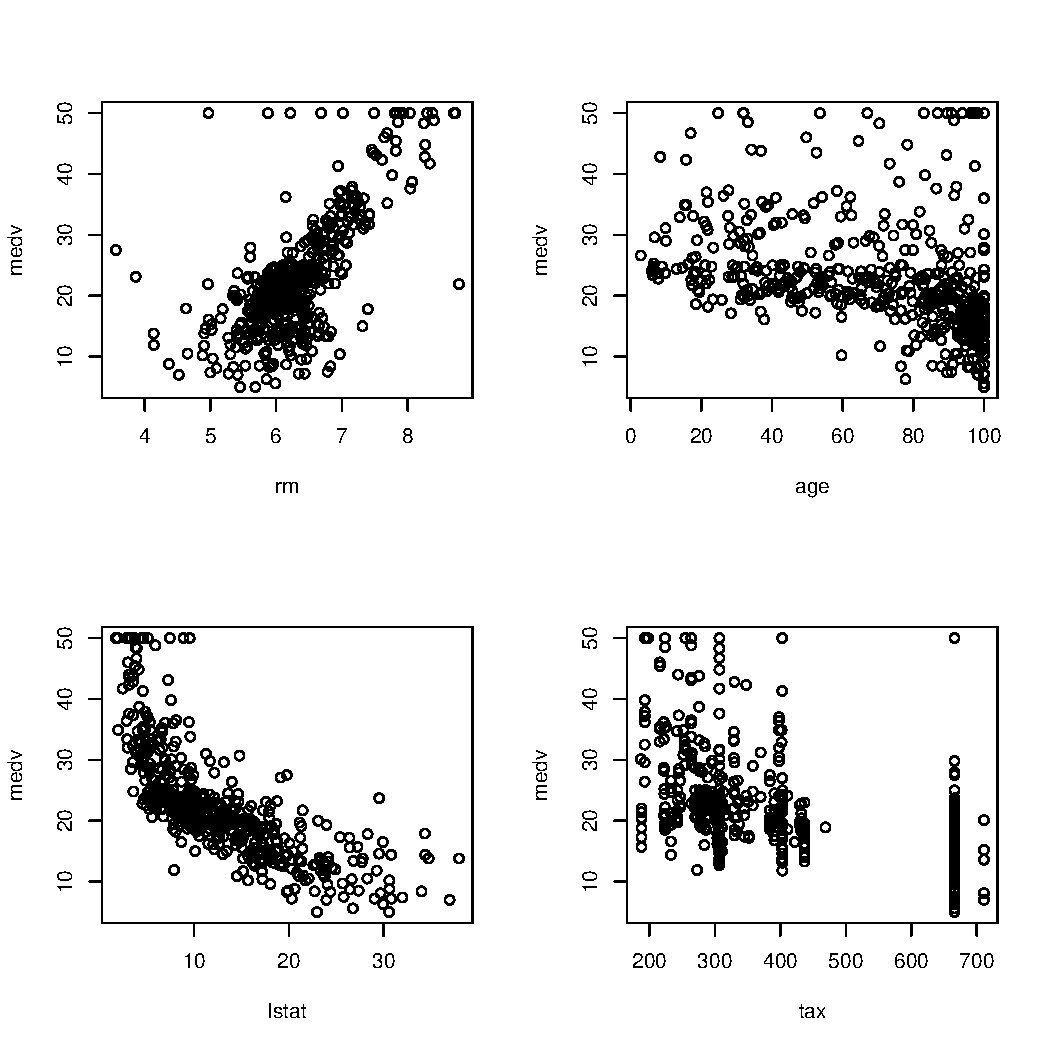
\includegraphics[width=\maxwidth]{figure/unnamed-chunk-20-1}

\end{knitrout}
        \caption{Relation entre la variable \texttt{medv} et les
          variables \texttt{rm}, \texttt{age}, \texttt{lstat} et
          \texttt{tax} des données \texttt{house.dat}}
        \label{fig:simple:house}
      \end{figure}
    \item Les résultats ci-dessous ont été obtenus avec \textsf{R}.
\begin{knitrout}
\definecolor{shadecolor}{rgb}{0.969, 0.969, 0.969}\color{fgcolor}\begin{kframe}
\begin{alltt}
\hlstd{fit1} \hlkwb{<-} \hlkwd{lm}\hlstd{(medv} \hlopt{~} \hlstd{rm,} \hlkwc{data} \hlstd{= house)}
\hlkwd{summary}\hlstd{(fit1)}
\end{alltt}
\begin{verbatim}
##
## Call:
## lm(formula = medv ~ rm, data = house)
##
## Residuals:
##     Min      1Q  Median      3Q     Max
## -23.346  -2.547   0.090   2.986  39.433
##
## Coefficients:
##             Estimate Std. Error t value Pr(>|t|)
## (Intercept)  -34.671      2.650  -13.08   <2e-16 ***
## rm             9.102      0.419   21.72   <2e-16 ***
## ---
## Signif. codes:
## 0 '***' 0.001 '**' 0.01 '*' 0.05 '.' 0.1 ' ' 1
##
## Residual standard error: 6.616 on 504 degrees of freedom
## Multiple R-squared:  0.4835,	Adjusted R-squared:  0.4825
## F-statistic: 471.8 on 1 and 504 DF,  p-value: < 2.2e-16
\end{verbatim}
\end{kframe}
\end{knitrout}
      On peut voir que tant l'ordonnée à l'origine que la pente sont
      très significativement différentes de zéro. La régression est
      donc elle-même significative. Cependant, le coefficient de
      détermination n'est que de $R^2 =
      0,4835$, %$
      ce qui indique que d'autres facteurs pourraient expliquer la
      variation dans \texttt{medv}.

      On calcule les bornes de l'intervalle de confiance de la
      régression avec la fonction \texttt{predict}:
\begin{knitrout}
\definecolor{shadecolor}{rgb}{0.969, 0.969, 0.969}\color{fgcolor}\begin{kframe}
\begin{alltt}
\hlstd{pred.ci} \hlkwb{<-} \hlkwd{predict}\hlstd{(fit1,} \hlkwc{interval} \hlstd{=} \hlstr{"confidence"}\hlstd{,} \hlkwc{level} \hlstd{=} \hlnum{0.95}\hlstd{)}
\end{alltt}
\end{kframe}
\end{knitrout}
      La droite de régression et ses bornes d'intervalle de confiance
      inférieure et supérieure sont illustrée à la figure
      \ref{fig:simple:house2}.
      \begin{figure}
        \centering
\begin{knitrout}
\definecolor{shadecolor}{rgb}{0.969, 0.969, 0.969}\color{fgcolor}\begin{kframe}
\begin{alltt}
\hlstd{ord} \hlkwb{<-} \hlkwd{order}\hlstd{(house}\hlopt{$}\hlstd{rm)}
\hlkwd{plot}\hlstd{(medv} \hlopt{~} \hlstd{rm,} \hlkwc{data} \hlstd{= house,} \hlkwc{ylim} \hlstd{=} \hlkwd{range}\hlstd{(pred.ci))}
\hlkwd{matplot}\hlstd{(house}\hlopt{$}\hlstd{rm[ord], pred.ci[ord,],}
        \hlkwc{type} \hlstd{=} \hlstr{"l"}\hlstd{,} \hlkwc{lty} \hlstd{=} \hlkwd{c}\hlstd{(}\hlnum{1}\hlstd{,} \hlnum{2}\hlstd{,} \hlnum{2}\hlstd{),} \hlkwc{lwd}\hlstd{=} \hlnum{2}\hlstd{,}
        \hlkwc{col} \hlstd{=} \hlstr{"black"}\hlstd{,} \hlkwc{add} \hlstd{=} \hlnum{TRUE}\hlstd{)}
\end{alltt}
\end{kframe}
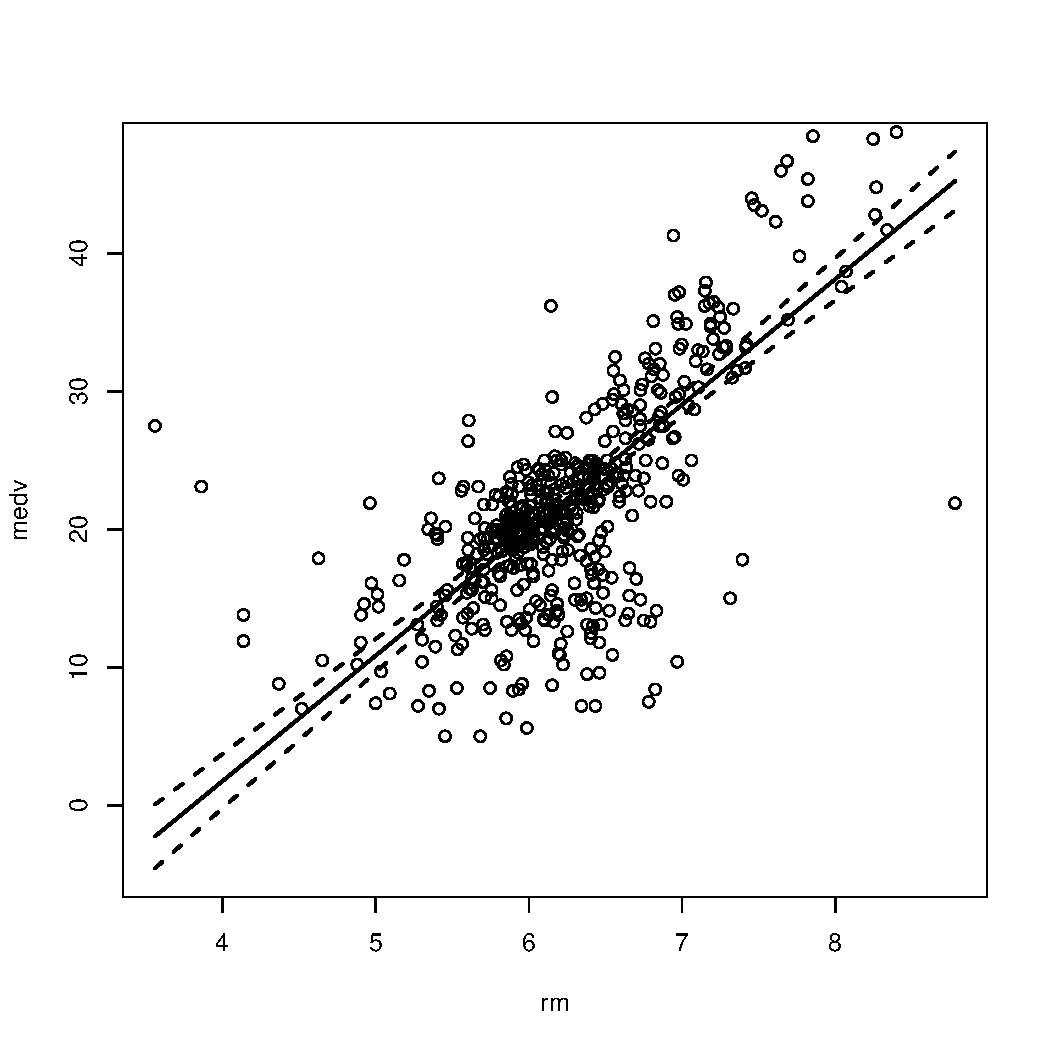
\includegraphics[width=\maxwidth]{figure/unnamed-chunk-23-1}

\end{knitrout}
        \caption{Résultat de la régression de la variable \texttt{rm} sur la variable \texttt{medv} des données \texttt{house.dat}}
        \label{fig:simple:house2}
      \end{figure}
    \item On reprend la même démarche, mais cette fois avec la
      variable \texttt{age}:
\begin{knitrout}
\definecolor{shadecolor}{rgb}{0.969, 0.969, 0.969}\color{fgcolor}\begin{kframe}
\begin{alltt}
\hlstd{fit2} \hlkwb{<-} \hlkwd{lm}\hlstd{(medv} \hlopt{~} \hlstd{age,} \hlkwc{data} \hlstd{= house)}
\hlkwd{summary}\hlstd{(fit2)}
\end{alltt}
\begin{verbatim}
##
## Call:
## lm(formula = medv ~ age, data = house)
##
## Residuals:
##     Min      1Q  Median      3Q     Max
## -15.097  -5.138  -1.958   2.397  31.338
##
## Coefficients:
##             Estimate Std. Error t value Pr(>|t|)
## (Intercept) 30.97868    0.99911  31.006   <2e-16 ***
## age         -0.12316    0.01348  -9.137   <2e-16 ***
## ---
## Signif. codes:
## 0 '***' 0.001 '**' 0.01 '*' 0.05 '.' 0.1 ' ' 1
##
## Residual standard error: 8.527 on 504 degrees of freedom
## Multiple R-squared:  0.1421,	Adjusted R-squared:  0.1404
## F-statistic: 83.48 on 1 and 504 DF,  p-value: < 2.2e-16
\end{verbatim}
\begin{alltt}
\hlstd{pred.ci} \hlkwb{<-} \hlkwd{predict}\hlstd{(fit2,} \hlkwc{interval} \hlstd{=} \hlstr{"confidence"}\hlstd{,} \hlkwc{level} \hlstd{=} \hlnum{0.95}\hlstd{)}
\end{alltt}
\end{kframe}
\end{knitrout}
      La régression est encore une fois très significative. Cependant,
      le $R^2$ est encore plus faible qu'avec la variable
      \texttt{rm}. Les variables \texttt{rm} et \texttt{age}
      contribuent donc chacune à expliquer les variations de la
      variable \texttt{medv} (et \texttt{rm} mieux que \texttt{age}),
      mais aucune ne sait le faire seule de manière satisfaisante. La
      droite de régression et l'intervalle de confiance de celle-ci
      sont reproduits à la figure \ref{fig:simple:house3}. On constate
      que l'intervalle de confiance est plus large qu'en b).
      \begin{figure}
        \centering
\begin{knitrout}
\definecolor{shadecolor}{rgb}{0.969, 0.969, 0.969}\color{fgcolor}\begin{kframe}
\begin{alltt}
\hlstd{ord} \hlkwb{<-} \hlkwd{order}\hlstd{(house}\hlopt{$}\hlstd{age)}
\hlkwd{plot}\hlstd{(medv} \hlopt{~} \hlstd{age,} \hlkwc{data} \hlstd{= house,} \hlkwc{ylim} \hlstd{=} \hlkwd{range}\hlstd{(pred.ci))}
\hlkwd{matplot}\hlstd{(house}\hlopt{$}\hlstd{age[ord], pred.ci[ord,],}
        \hlkwc{type} \hlstd{=} \hlstr{"l"}\hlstd{,} \hlkwc{lty} \hlstd{=} \hlkwd{c}\hlstd{(}\hlnum{1}\hlstd{,} \hlnum{2}\hlstd{,} \hlnum{2}\hlstd{),} \hlkwc{lwd} \hlstd{=} \hlnum{2}\hlstd{,}
        \hlkwc{col} \hlstd{=} \hlstr{"black"}\hlstd{,} \hlkwc{add} \hlstd{=} \hlnum{TRUE}\hlstd{)}
\end{alltt}
\end{kframe}
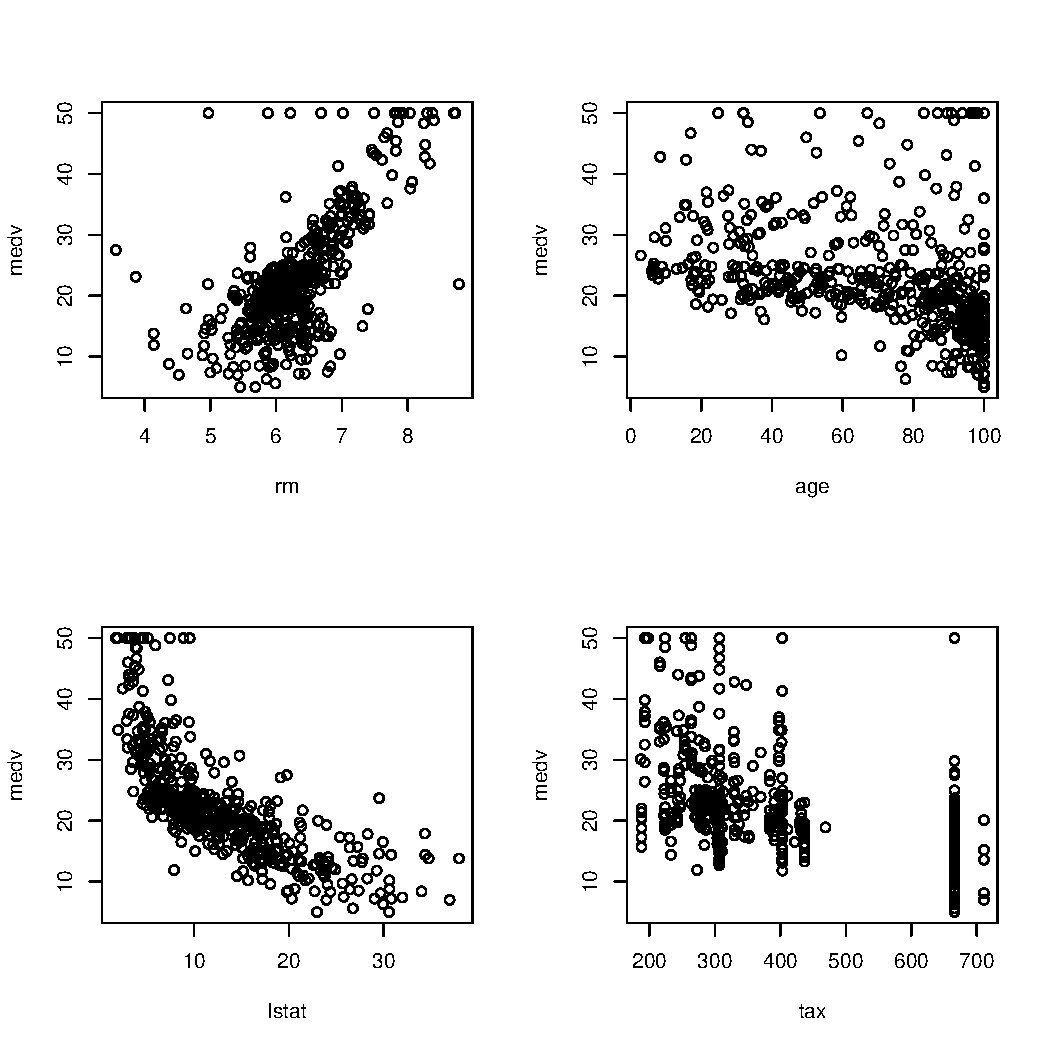
\includegraphics[width=\maxwidth]{figure/unnamed-chunk-25-1}

\end{knitrout}
        \caption{Résultat de la régression de la variable \texttt{age} sur la variable \texttt{medv} des données \texttt{house.dat}}
        \label{fig:simple:house3}
      \end{figure}
    \end{enumerate}
  
\end{solution}
\begin{solution}{2.18}
    \begin{enumerate}
    \item On importe les données dans \textsf{R}, puis on effectue les
      conversions demandées. La variable \texttt{consommation}
      contient la consommation des voitures en $\ell$/100~km et la
      variable \texttt{poids} le poids en kilogrammes.
\begin{knitrout}
\definecolor{shadecolor}{rgb}{0.969, 0.969, 0.969}\color{fgcolor}\begin{kframe}
\begin{alltt}
\hlstd{carburant} \hlkwb{<-} \hlkwd{read.table}\hlstd{(}\hlstr{"carburant.dat"}\hlstd{,} \hlkwc{header} \hlstd{=} \hlnum{TRUE}\hlstd{)}
\hlstd{consommation} \hlkwb{<-} \hlnum{235.1954}\hlopt{/}\hlstd{carburant}\hlopt{$}\hlstd{mpg}
\hlstd{poids} \hlkwb{<-} \hlstd{carburant}\hlopt{$}\hlstd{poids} \hlopt{*} \hlnum{0.45455} \hlopt{*} \hlnum{1000}
\end{alltt}
\end{kframe}
\end{knitrout}
    \item La fonction \texttt{summary} fournit l'information
      essentielle pour juger de la validité et de la qualité du
      modèle:
\begin{knitrout}
\definecolor{shadecolor}{rgb}{0.969, 0.969, 0.969}\color{fgcolor}\begin{kframe}
\begin{alltt}
\hlstd{fit} \hlkwb{<-} \hlkwd{lm}\hlstd{(consommation} \hlopt{~} \hlstd{poids)}
\hlkwd{summary}\hlstd{(fit)}
\end{alltt}
\begin{verbatim}
##
## Call:
## lm(formula = consommation ~ poids)
##
## Residuals:
##      Min       1Q   Median       3Q      Max
## -2.07123 -0.68380  0.01488  0.44802  2.66234
##
## Coefficients:
##               Estimate Std. Error t value Pr(>|t|)
## (Intercept) -0.0146530  0.7118445  -0.021    0.984
## poids        0.0078382  0.0005315  14.748   <2e-16 ***
## ---
## Signif. codes:
## 0 '***' 0.001 '**' 0.01 '*' 0.05 '.' 0.1 ' ' 1
##
## Residual standard error: 1.039 on 36 degrees of freedom
## Multiple R-squared:  0.858,	Adjusted R-squared:  0.854
## F-statistic: 217.5 on 1 and 36 DF,  p-value: < 2.2e-16
\end{verbatim}
\end{kframe}
\end{knitrout}
      Le modèle est donc le suivant: $Y_t =
      -0,01465 +
      0,007838 X_t +
      \varepsilon_t$, $\varepsilon_t \sim N(0,
      1,039^2)$, où $Y_t$ est la
      consommation en litres aux 100 kilomètres et $X_t$ le poids en
      kilogrammes. La faible valeur $p$ du test $F$ indique une
      régression très significative. De plus, le $R^2$ de
      0,858 %$
      confirme que l'ajustement du modèle est assez bon.
    \item On veut calculer un intervalle de confiance pour la
      consommation en carburant prévue d'une voiture de
      \nombre{1350}~kg. On obtient, avec la fonction \texttt{predict}:
\begin{knitrout}
\definecolor{shadecolor}{rgb}{0.969, 0.969, 0.969}\color{fgcolor}\begin{kframe}
\begin{alltt}
\hlkwd{predict}\hlstd{(fit,} \hlkwc{newdata} \hlstd{=} \hlkwd{data.frame}\hlstd{(}\hlkwc{poids} \hlstd{=} \hlnum{1350}\hlstd{),} \hlkwc{interval} \hlstd{=} \hlstr{"prediction"}\hlstd{)}
\end{alltt}
\begin{verbatim}
##       fit      lwr     upr
## 1 10.5669 8.432089 12.7017
\end{verbatim}
\end{kframe}
\end{knitrout}
    \end{enumerate}
  
\end{solution}
